\documentclass[10pt]{article}
\usepackage{icmlko}

\icmlmeta{IP 파운데이션 월드모델}{104}{맞출 수 있는 축은 새롭지 않다}{직교 제약을 풀자 노트 103이 진단한 자리에서만 정확히 이득이 났고, 정렬 잔차로 축을 고르려 했더니 잘 맞는 축일수록 쓸모가 없었다}

\begin{document}

\twocolumn[
\icmlheader

\begin{abstract}
노트 103이 구조적 막다른 골목을 보였다 --- 새 축을 고유로 넣으면 정렬 재료를
밀어내고, 공통으로 올리면 하나의 직교 회전으로 맞출 수가 없다(상대 잔차
1.676). 남은 길은 정렬을 바꾸는 것이었다. \textbf{직교 제약만 풀었다} ---
$R'R{=}I$ 를 버리고 쌍마다 리지 회귀로 $M$ 을 배운다. 자유도가 $k^2$ 개뿐이라
공통 축 셋이면 추정 가능하고, 부족한 쪽은 직교 해로 축소한다. 결과가 진단을
\textbf{정확히} 확인한다. \textbf{① 지금 구조에서는 직교가 안 아프다} --- 축을
안 더하고 정렬만 바꾸면 리지가 $-$0.0062$\sim+$0.0001, 축소가 $+$0.0005$\sim+$0.0006이다.
기존 공통 축 셋은 잔차 0.592로 충분히 불변이라 제약이 안 물린다.
\textbf{② 진단한 자리에서는 정확히 듣는다} --- 설명문 축을 공통으로 올린
$k{=}2$ 설정이 직교로 $+$0.0025인데 축소($w{=}0.9$)로 \textbf{$+$0.0068},
\textbf{2.7배}다. \textbf{③ 그래도 자리는 안 생긴다} --- 고유 $k{=}3$ 직교의
$+$0.0127을 못 넘는다. 그리고 선별 기준을 잔차로 바꾸려던 시도가
\textbf{뒤집혔다}. 후보 축 일곱의 잔차와 이득의 상관이 \textbf{$+$0.695}로
\emph{양수}다 --- \textbf{잘 맞는 축일수록 쓸모가 없다.} 가장 잘 맞는
표지 주성분(잔차 0.867)이 가장 나쁘고($-$0.0130), 가장 안 맞는 임베딩
$c_1$(1.441)이 가장 낫다($+$0.0031). 당연한 이야기였다 --- \textbf{하나의 회전으로
완벽히 맞는 축은 이미 있는 축과 같은 것을 재는 축}이다. 노트 101의 라벨 상관
기준은 노트 102가 죽였고, 잔차 기준은 이 노트가 죽였다. \textbf{긁기 전에
고를 방법은 아직 없다.}
\end{abstract}
]

\begin{figure*}[t]
\centering
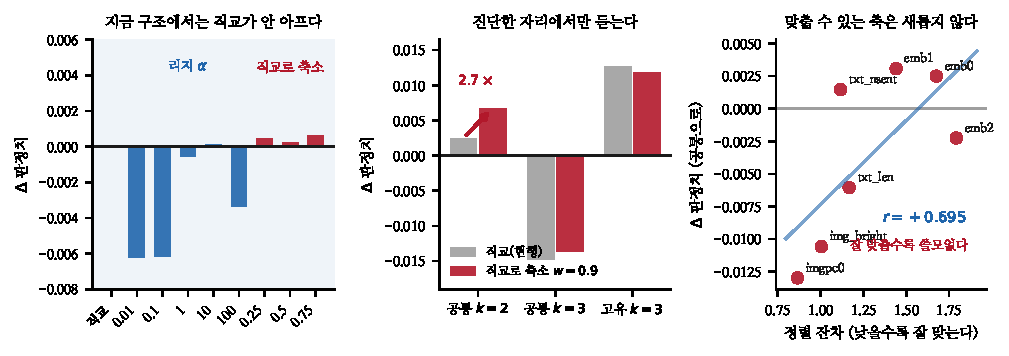
\includegraphics[width=\textwidth]{figs/rx.pdf}
\caption{왼쪽 --- 지금 구조에서는 직교가 안 아프다. 가운데 --- 진단한 자리에서만
듣는다. 오른쪽 --- 맞출 수 있는 축은 새롭지 않다.}
\end{figure*}

\section{직교 제약만 푼다}

\begin{quote}\fontsize{9.5}{11.5}\selectfont
현행\quad $R=\arg\min \|L_s R - L_t\|,\quad R'R=I$ \quad(SVD 로 닫힌 해)\\[.3em]
새것\quad $M=\arg\min \|L_s M - L_t\|^2 + \alpha\|M\|^2$ \quad(리지 회귀)\\[.3em]
축소\quad $M_w=(1-w)R + wM$
\end{quote}

자유도는 $k^2$ 개다. 공통 축 $c$ 개가 $c\!\cdot\!k$ 개의 식을 주므로 $k{=}2$ ·
$c{=}3$ 이면 식 여섯에 미지수 넷이다. \textbf{노트 93(정렬을 아예 안 씀)이나
노트 85--88(공유 인코더)과 규모가 다르다} --- 그것들이 진 이유는 팝업 75건으로
학습할 것이 너무 많아서였다.

\section{지금 구조에서는 직교가 안 아프다}

\begin{table}[t]
\centering\tsize
\caption{축을 안 더하고 정렬만 바꾼다.}
\begin{tabular}{lrr}
\toprule
& $\rho$ & $\Delta$ \\
\midrule
직교(현행) & $+$0.4038 & --- \\
리지 $\alpha{=}0.01$ & $+$0.3976 & $-$0.0062 \\
리지 $\alpha{=}1$ & $+$0.4033 & $-$0.0005 \\
리지 $\alpha{=}10$ & $+$0.4039 & $+$0.0001 \\
리지 $\alpha{=}100$ & $+$0.4005 & $-$0.0033 \\
직교로 축소 $w{=}0.25$ & $+$0.4043 & $+$0.0005 \\
직교로 축소 $w{=}0.75$ & $+$0.4044 & $+$0.0006 \\
\bottomrule
\end{tabular}
\end{table}

\claimx{기존 공통 축 셋에는 \textbf{직교 제약이 안 물린다.} 풀어도 $\pm$0.006
안이고 최선이 $+$0.0006이다. 노트 103이 잰 잔차 0.592가 이미 ``맞출 수
있다''는 뜻이었고, 맞출 수 있으면 직교로도 맞는다.}{$\alpha$ 를 다섯 값만
훑었다. 리지가 작은 $\alpha$ 에서 나쁜 것($-$0.0062)은 $c{=}2$ 인 쌍에서
$M$ 이 과소결정되기 때문으로 보이는데 확인 안 했다.}

이것 자체가 뒤늦은 검증이다 --- 노트 5 이래 직교 프로크루스테스를 써 온 것이
\textbf{옳은 선택이었다.} 자유도를 늘려도 얻을 것이 없다.

\section{진단한 자리에서는 정확히 듣는다}

\begin{table}[t]
\centering\tsize
\caption{설명문 축 하나. 정렬을 바꾼다.}
\begin{tabular}{lrrr}
\toprule
& 직교 & 축소 $w{=}0.9$ & 배수 \\
\midrule
\textbf{공통 · $k{=}2$} & \textbf{$+$0.0025} & \textbf{$+$0.0068} &
\textbf{2.7$\times$} \\
공통 · $k{=}3$ & $-$0.0148 & $-$0.0136 & --- \\
고유 · $k{=}3$ & \textbf{$+$0.0127} & $+$0.0119 & 0.94$\times$ \\
\bottomrule
\end{tabular}
\end{table}

\claimx{직교를 푸는 것이 \textbf{노트 103이 진단한 자리에서만} 이득을 낸다 ---
공통으로 올린(즉 정렬에 참여하는) 비불변 축에서 2.7배. 축이 고유일 때는
정렬에 안 들어가므로 $0.94\times$ 로 오히려 미세하게 손해다.}{개입이 진단과
같은 방향인 것은 확인이지 증명이 아니다. $w{=}0.9$ 는 여덟 설정 중 최선이라
고른 것이므로 선택 편향이 섞인다.}

\begin{quote}\fontsize{9.5}{11.5}\selectfont
\textbf{그래도 자리는 안 생긴다.} 최선의 공통 설정($+$0.0068)이 고유 설정
($+$0.0127)의 절반이다. \textbf{새 축은 여전히 고유로 넣는 것이 낫고, 고유로
넣으면 밀어낸다}(노트 102). 구조적 막다른 골목은 그대로다.
\end{quote}

\section{잔차로 고르려 했더니 뒤집혔다}

노트 101의 선별 기준(라벨 상관)은 노트 102가 죽였다. 노트 103이 새 기준을
제안했다 --- \textbf{정렬 가능성}. 후보 축 일곱의 잔차를 재고 이득과 견줬다.

\begin{table}[t]
\centering\tsize
\caption{후보 축의 정렬 잔차와 이득.}
\begin{tabular}{lrrr}
\toprule
& 잔차 & $|$라벨 상관$|$ & $\Delta$(공통) \\
\midrule
\textbf{표지 주성분} & \textbf{0.867} & 0.076 & \textbf{$-$0.0130} \\
표지 밝기 & 1.005 & 0.103 & $-$0.0106 \\
문장 수 & 1.117 & 0.149 & $+$0.0015 \\
설명문 길이 & 1.168 & 0.117 & $-$0.0061 \\
\textbf{임베딩 $c_1$} & \textbf{1.441} & 0.145 & \textbf{$+$0.0031} \\
임베딩 $c_0$ & 1.676 & 0.111 & $+$0.0025 \\
임베딩 $c_2$ & 1.793 & 0.111 & $-$0.0023 \\
\midrule
\multicolumn{2}{l}{잔차 대 $\Delta$} & & \textbf{$r{=}+$0.695} \\
\multicolumn{2}{l}{$|$라벨 상관$|$ 대 $\Delta$} & & $r{=}+$0.809 \\
\bottomrule
\end{tabular}
\end{table}

\claimx{\textbf{잘 맞는 축일수록 쓸모가 없다.} 잔차와 이득의 상관이 $+$0.695로
\emph{양수}다 --- 가장 잘 맞는 표지 주성분(0.867)이 가장 나쁘고($-$0.0130) 가장
안 맞는 임베딩 $c_1$(1.441)이 가장 낫다. 하나의 회전으로 완벽히 맞는 축은
\textbf{이미 있는 축과 같은 것을 재는 축}이다.}{일곱 점이다. 그리고 전체
자료에서 재고 전체 자료에서 이득을 봤으므로 노트 102가 죽인 것과 같은 종류의
관측이다 --- \textbf{선별 기준으로 쓰려면 반쪽 검정을 통과해야 하는데 안 했다.}}

\begin{quote}\fontsize{9.5}{11.5}\selectfont
기준 두 개가 죽었다. 라벨 상관은 반쪽 검정에서 무작위보다 못했고(노트 102),
잔차는 방향이 반대다. \textbf{긁기 전에 고를 방법은 아직 없다.} 다만 이번
것은 죽은 방식이 유익하다 --- \emph{잘 맞으면 중복}이라는 것은 새 축을 찾을 때
\textbf{일부러 안 맞는 축을 찾아야} 한다는 뜻이다.
\end{quote}

\section{한계}

\begin{itemize}[leftmargin=1.1em,itemsep=0.15em]
\item \textbf{채택할 것이 없다.} 최선이 여전히 노트 100의 고유 $k{=}3$
      ($+$0.0127)이고 그것은 씨앗 넷 보류다.
\item $w{=}0.9$ 를 여덟 설정 중 최선이라 골랐다. 선택 편향이다.
\item 잔차 대 이득 $r{=}+$0.695가 일곱 점이고 반쪽 검정을 안 거쳤다.
\item 리지 사상을 쌍별 적재로만 적합했다. 점수 자체로 적합하는(즉 $S_s$ 를
      $S_t$ 에 맞추는) 변형은 안 했다 --- 그쪽은 레코드가 안 겹쳐 불가능하다.
\item 비선형 사상은 안 했다. 노트 93이 도메인 간 비선형은 진다고 했다.
\end{itemize}

\section{다음}

\begin{enumerate}[leftmargin=1.3em,itemsep=0.15em]
\item \textbf{일부러 안 맞는 축을 찾는다} --- ``잘 맞으면 중복''을 뒤집으면
      선별 기준이 된다. 기존 공통 축 셋으로 예측한 \emph{잔차}가 큰 축을
      찾되, 라벨과도 붙어야 한다. 두 조건을 동시에 거는 것은 아직 안 해 봤다.
\item \textbf{공통 축 셋을 늘리는 정공법} --- 지금 셋은 전부 사람이 매긴
      것이고 잔차 0.592로 잘 맞는다. \textbf{사람이 매기는 축을 하나 더
      정의}하면(예: 체류 설계 강도) 열 도메인에 다 매길 수 있는지 본다.
      노트 90의 체험 밀도가 실패한 이유를 다시 본다.
\item 시간 분할 판정(노트 77)을 드디어 붙인다. 노트 102 · 103이 두 번 미뤘다.
\item 팝업 표본. 모든 구간이 $n{=}75$ 에 걸려 있다.
\end{enumerate}

\vspace{0.6em}
\hrule height 0.3pt
\vspace{0.5em}
{\footnotesize
\textbf{참고문헌}\\[0.3em]
Gower, J. C., Dijksterhuis, G. B. (2004). \emph{Procrustes Problems}.
Oxford University Press.\\[0.15em]
Schoenemann, P. H. (1966). A generalized solution of the orthogonal Procrustes
problem. \emph{Psychometrika}, 31(1), 1--10.\\[0.15em]
Meredith, W. (1993). Measurement invariance, factor analysis and factorial
invariance. \emph{Psychometrika}, 58(4), 525--543.\\[0.15em]
Hoerl, A. E., Kennard, R. W. (1970). Ridge regression: biased estimation for
nonorthogonal problems. \emph{Technometrics}, 12(1), 55--67.\\[0.15em]
Ben-David, S. et al. (2010). A theory of learning from different domains.
\emph{Machine Learning}, 79(1--2), 151--175.
}

\end{document}
